%%
% TUM Corporate Design LaTeX Templates
% Based on the templates from https://www.tum.de/cd
%
% Feel free to join development on
% https://gitlab.lrz.de/tum-templates/templates
% and/or to create an issue in case of trouble.
%
% tum-presentation class for scientific talks, thesis presentations, ...
%
%%

%\documentclass[4to3]{tum-presentation}
%\documentclass[navsym]{tum-presentation}
%\documentclass[nothreeliner]{tum-presentation}
%\documentclass[handout,4on1]{tum-presentation}
%\documentclass[handout,2on1]{tum-presentation}
%\documentclass[handout]{tum-presentation}
\documentclass{tum-presentation}

\addbibresource{literature.bib}


\title[Shortened Title]{Learning to Encode Text as Human-Readable Summaries}
\subtitle{Generative Adversarial Networks}
\author[]{\textbf{Denys Lazarenko}\inst{1}, Author 2\inst{2}}
\institute[]{\inst{1} Department of Mathematics ,
  Technical University of Munich (TUM)\\
  \inst{2} Department of Informatics, Technical University of Munich (TUM)}
\date{Seminar Course - Adversarial and Secure Machine Learning}

\footline{\insertshortauthor~|~\insertshorttitle}

\begin{document}

\begin{frame}[noframenumbering]
  \titlepage
\end{frame}

\begin{frame}
  \frametitle{Motivation}


  \footfullcite{jirauschek2014}
\end{frame}

\begin{frame}
	\frametitle{Outline}
	\begin{enumerate}
		\item Overview of the problem
		\begin{itemize}
			\item Main result
			\item Problem setup
			\item What was actually implemented from the paper
		\end{itemize}
		\item Dataset
		\begin{itemize}
			\item Quantitive analysis
			\item Data preprocessing
		\end{itemize}
		\item Pointer-generator network 
		\begin{itemize}
			\item Encoder-decoder architectur
			\item Attention mechanism
			\item Summarization 
			\begin{itemize}
				\item State of the art
				\item Implementation
			\end{itemize}
		\end{itemize}
		\item Wasserstein Generative Adversarial Networks(WGAN) 
		\begin{itemize}
			\item General Theory behind GANs
			\item From GAN to WGAN
			\item Problem while training GANs
		\end{itemize}	
		\item Results
		\item Future work
	\end{enumerate}
\end{frame}

\begin{frame}
	\frametitle{Overview}
	\begin{figure}
		\centering
		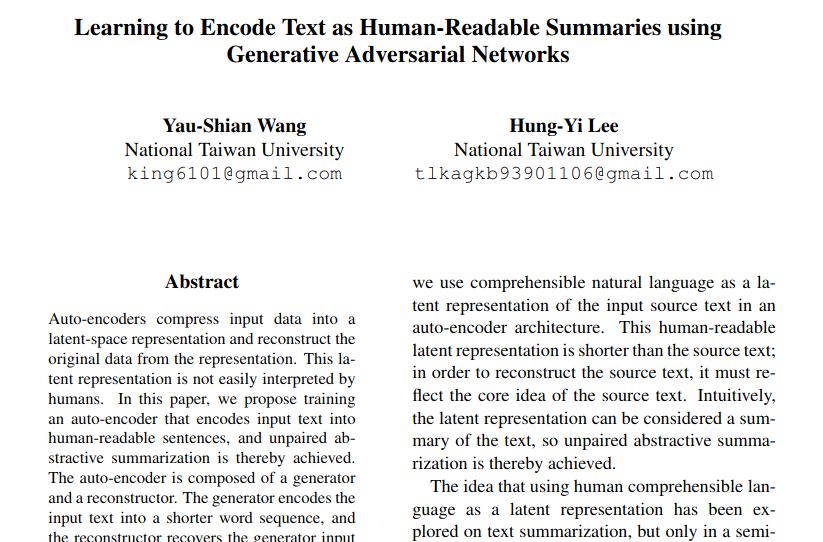
\includegraphics[width=0.65\textwidth,keepaspectratio=true]{tum-resources/images/paper_1.png}
		\label{fig:paper_1}
	\end{figure}
\end{frame}

\begin{frame}
	\frametitle{Assumptions}
	\begin{itemize}
		\item CNN dataset
		\item Unpaired WGAN model
		\item 5000 words in vocabulary (Pointer model)
		\item without coverage mechanism (Pointer model)
		\item ...
	\end{itemize}
\end{frame}

\begin{frame}
	\begin{figure}
		\centering
		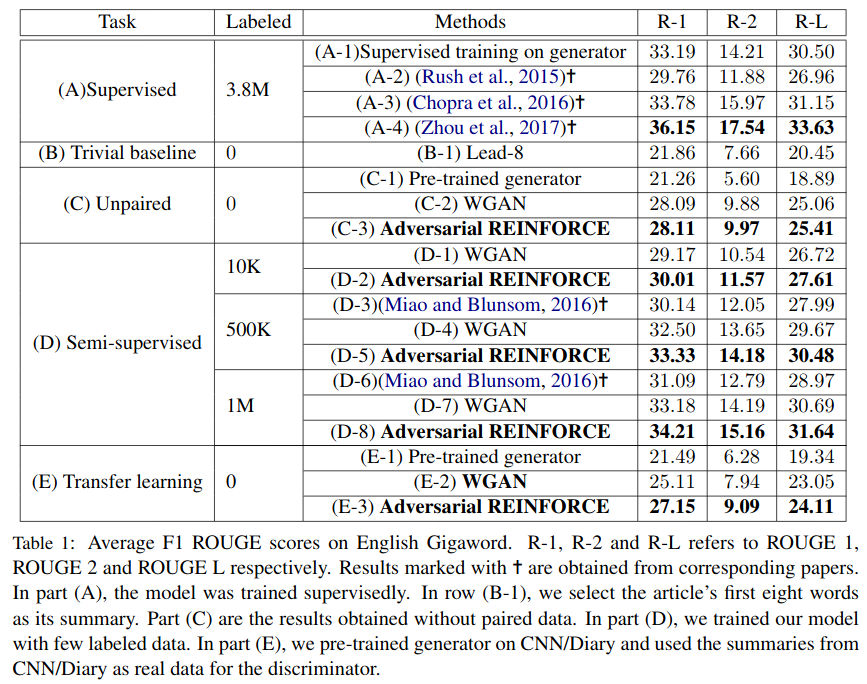
\includegraphics[width=0.6\textwidth,keepaspectratio=true]{tum-resources/images/paper_4.png}
		\label{fig:paper_4}
	\end{figure}
\end{frame}

\begin{frame}
	\frametitle{CNN / Daily Mail dataset}
	\begin{figure}
	\centering
	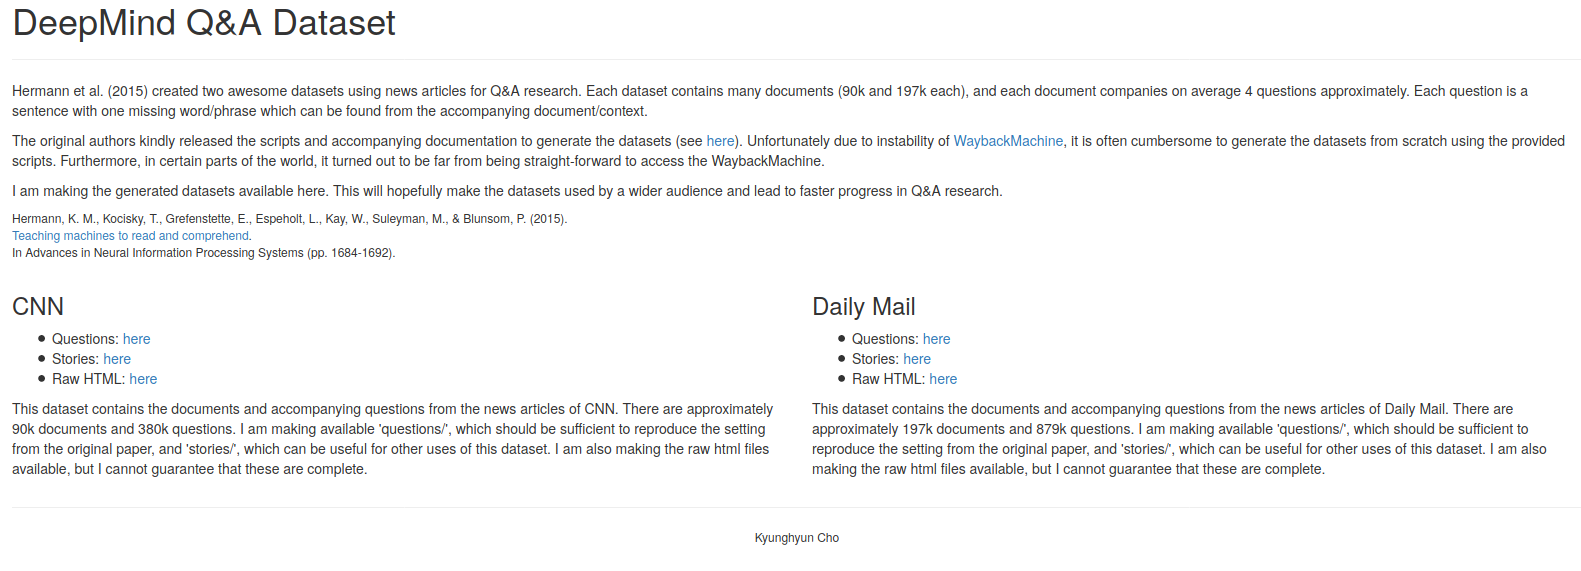
\includegraphics[width=1\textwidth,keepaspectratio=true]{tum-resources/images/dataset_1.png}
	\label{fig:dataset_1}
	\end{figure}
\end{frame}

\begin{frame}
	\frametitle{CNN / Daily Mail dataset}
	\begin{figure}
		\centering
		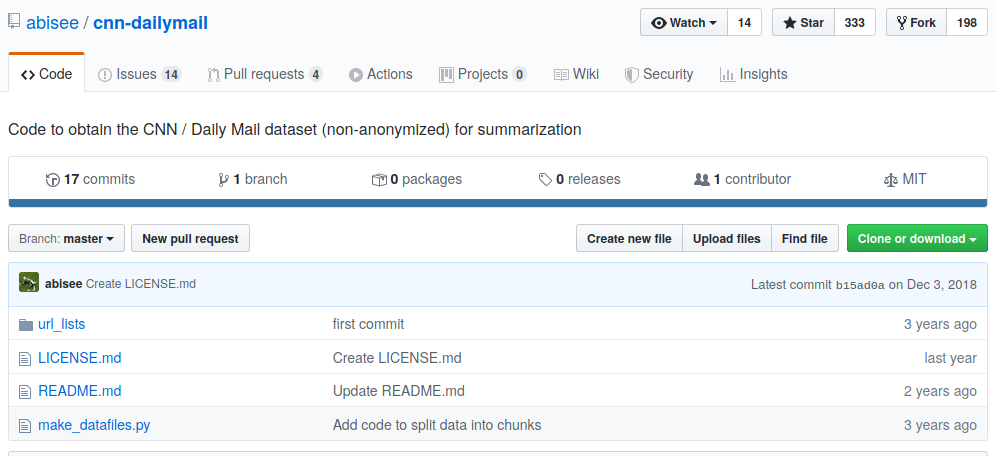
\includegraphics[width=0.95\textwidth,keepaspectratio=true]{tum-resources/images/dataset_2.png}
		\label{fig:dataset_2}
	\end{figure}
\end{frame}

\begin{frame}
	\frametitle{Load Dataset}
	\begin{figure}
		\centering
		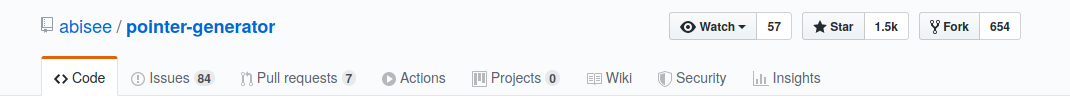
\includegraphics[width=0.95\textwidth,keepaspectratio=true]{tum-resources/images/dataset_3.png}
		\label{fig:dataset_3}
		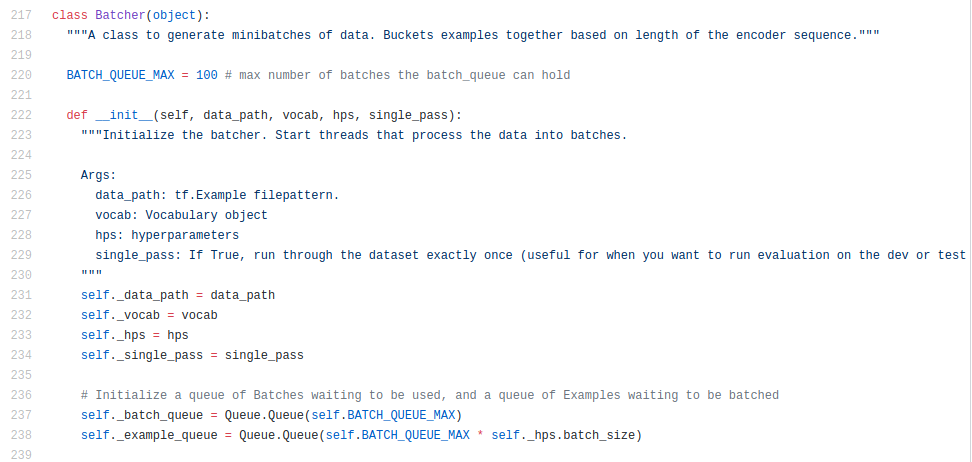
\includegraphics[width=0.95\textwidth,keepaspectratio=true]{tum-resources/images/dataset_4.png}
		\label{fig:dataset_4}
	\end{figure}
\end{frame}

\begin{frame}[c]
	\centering
	\begin{center}
		\Huge\textbf{Encode-decoder architectur}
	\end{center}
\end{frame}

\begin{frame}
  \frametitle{Sequence to sequence}
	\begin{figure}
		\centering
		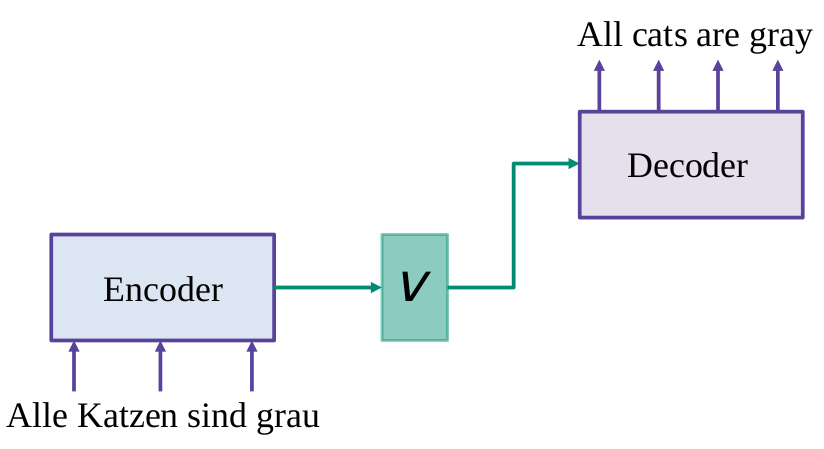
\includegraphics[width=0.65\textwidth,keepaspectratio=true]{tum-resources/images/seq2seq_1.png}
		\label{fig:seq2seq_1}
	\end{figure}
	\begin{flushright}
		\textit{	From "Natural Language Processing", A. Potapenko et.al. HSE, 2019. }
	\end{flushright}
\end{frame}

\begin{frame}
	\frametitle{Sequence to sequence}
	\begin{figure}
		\centering
		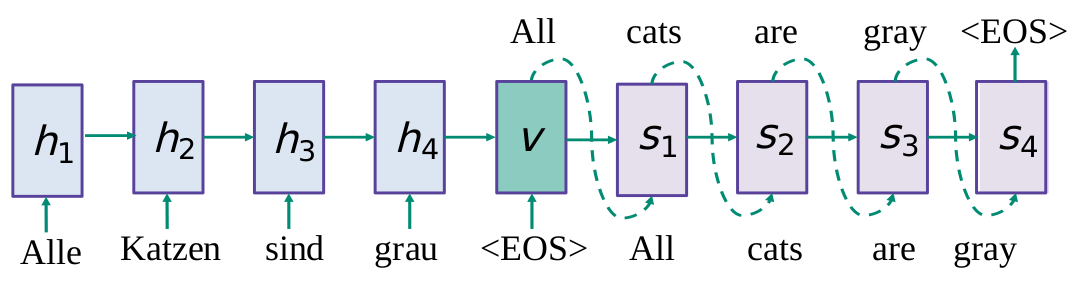
\includegraphics[width=0.65\textwidth,keepaspectratio=true]{tum-resources/images/seq2seq_2.png}
		\label{fig:seq2seq_2}
	\end{figure}
	\begin{flushright}
		\textit{	From "Natural Language Processing", A. Potapenko et.al. HSE, 2019. }
	\end{flushright}
\end{frame}

\begin{frame}
	\frametitle{Sequence to sequence}
	\begin{figure}
		\centering
		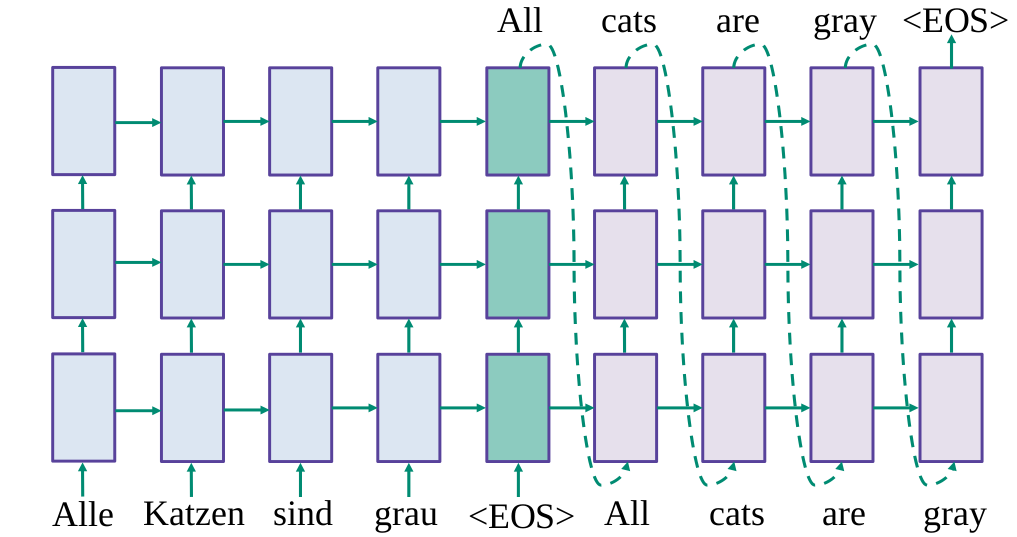
\includegraphics[width=0.65\textwidth,keepaspectratio=true]{tum-resources/images/seq2seq_3.png}
		\label{fig:seq2seq_3}
	\end{figure}
	\begin{flushright}
	\textit{	From "Natural Language Processing", A. Potapenko et.al. HSE, 2019. }
	\end{flushright}

\end{frame}

\begin{frame}
	\frametitle{Sequence to sequence}
	\begin{figure}
		\centering
		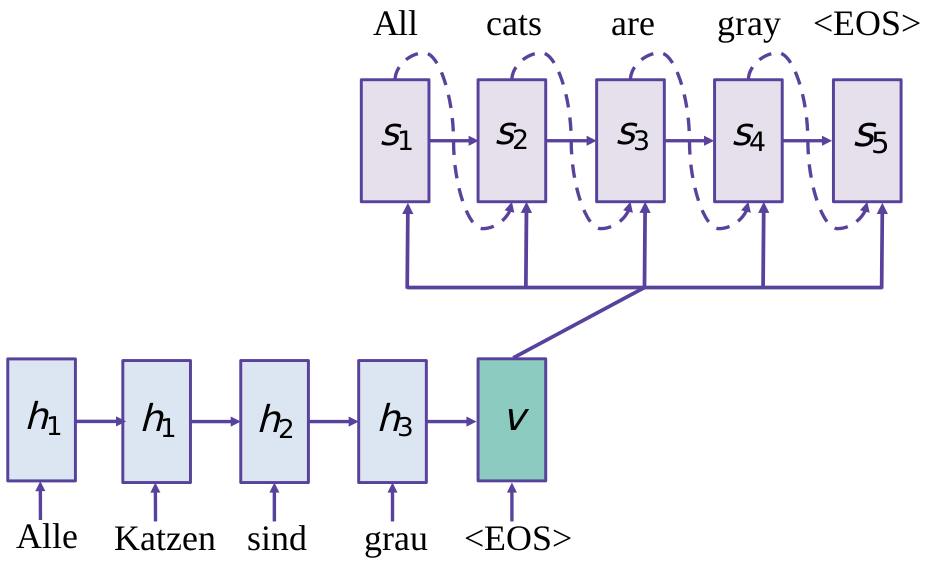
\includegraphics[width=0.65\textwidth,keepaspectratio=true]{tum-resources/images/seq2seq_4.png}
		\label{fig:seq2seq_4}
	\end{figure}
	\begin{flushright}
	\textit{	From "Natural Language Processing", A. Potapenko et.al. HSE, 2019. }
	\end{flushright}
\end{frame}

\begin{frame}
	\centering \huge $\mathbb{P}\left[ y_{1}, \dots y_{J} | x_1, \dots, x_I \right] = 
	\prod_{j=1}^{J} \mathbb{P}\left[ y_{j} |  \textcolor{red}{v}, y_1, \dots, y_{j-1}\right]$
	\begin{itemize}
		\item \textbf{\textcolor{TUMBlau}{Encoder:}} maps the source sequence to the hidden vector
		$RNN: h_i = f(h_{i-1}, x_i)$, where $\textcolor{red}{v=h_I}$
		\item \textbf{\textcolor{TUMBlau}{Decoder:}} performs language modeling given this vector
		$RNN: s_j=g(s_{j-1}, [y_{j-1}, \textcolor{red}{v}])$
		\item \textbf{\textcolor{TUMBlau}{Prediction:}}
		$\mathbb{P}\left[ y_{j} |  \textcolor{red}{v}, y_1, \dots, y_{j-1}\right] = softmax(Us_j + b)$
	\end{itemize}	
	\begin{flushright}
	\textit{	From "Natural Language Processing", A. Potapenko et.al. HSE, 2019. }
	\end{flushright}
\end{frame}
	
\begin{frame}
	\frametitle{Sequence to sequence}
	\begin{figure}
		\centering
		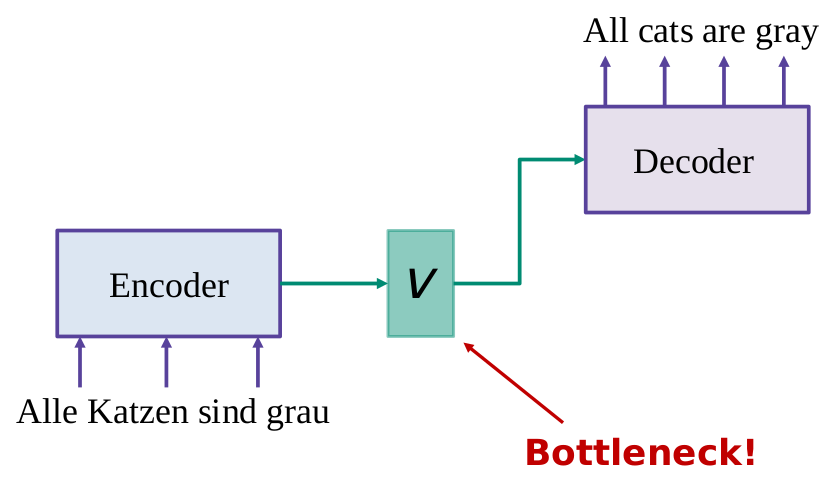
\includegraphics[width=0.65\textwidth,keepaspectratio=true]{tum-resources/images/seq2seq_5.png}
		\label{fig:seq2seq_5}
	\end{figure}
	\begin{flushright}
	\textit{	From "Natural Language Processing", A. Potapenko et.al. HSE, 2019. }
	\end{flushright}
\end{frame}

\begin{frame}[c]
	\centering
	\begin{center}
		\Huge\textbf{Attention mechanism}
	\end{center}
\end{frame}

\begin{frame}
	\frametitle{Attention mechanism}
	\begin{figure}
		\centering
		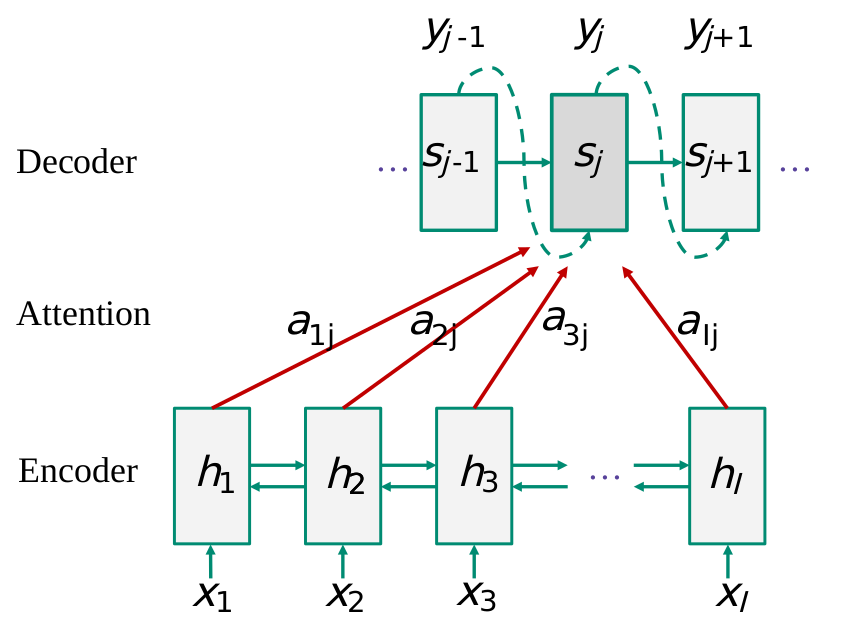
\includegraphics[width=0.6\textwidth,keepaspectratio=true]{tum-resources/images/att_1.png}
		\label{fig:att_1}
	\end{figure}
	\begin{flushright}
	\textit{	From "Natural Language Processing", A. Potapenko et.al. HSE, 2019. }
	\end{flushright}
\end{frame}

\begin{frame}
	\begin{itemize}
		\vskip 0.2in
		\centering \huge \item Encoder states are weighted to obtain the representation relevant to the decoder state:\\
		\vskip 0.2in
		$\textcolor{TUMBlau}{v_j=\sum_{i=1}^{I} \alpha_{ij} h_i}$
		\vskip 0.2in
		\item The weights are learnt and should find the most
		relevant encoder positions:\\
		\vskip 0.2in
		$\alpha_{ij} = \dfrac{exp\textcolor{TUMBlau}{(sim(h_i, s_{j-1}))}}{\sum_{i^{'}}^{I} exp(\textcolor{TUMBlau}{sim(h_{i^{'}}, s_{j-1}))}}$
	\end{itemize}	
	\begin{flushright}
	\textit{	From "Natural Language Processing", A. Potapenko et.al. HSE, 2019. }
	\end{flushright}
\end{frame}

\begin{frame}
	\begin{itemize}
	\huge\item \textbf{\textcolor{TUMBlau}{Additive attention:}}
	\begin{center}
			$sim(h_i, s_j)=w^T \tanh(W_h h_i + W_s s_j)$
	\end{center}
	\vskip 0.2in
	\item \textbf{\textcolor{TUMBlau}{Multiplicative attention:}}
	\begin{center}
	$sim(h_i, s_j)=h_i^T Ws_j$
	\end{center}
	\vskip 0.2in
	\item \textbf{\textcolor{TUMBlau}{Dot product also works:}}
	\begin{center}
	$sim(h_i, s_j)=h_i^T s_j$
	\end{center}	
\end{itemize}	
	\begin{flushright}
	\textit{	From "Natural Language Processing", A. Potapenko et.al. HSE, 2019. }
	\end{flushright}
\end{frame}

\begin{frame}
	\frametitle{Put all together}
	\vskip 0.5in
	\centering \huge $\mathbb{P}\left[ y_{1}, \dots y_{J} | x_1, \dots, x_I \right] = 
	\prod_{j=1}^{J} \mathbb{P}\left[ y_{j} |  \textcolor{red}{v_j}, y_1, \dots, y_{j-1}\right]$
	\begin{itemize}
		\vskip 0.5in
		\item \textbf{\textcolor{TUMBlau}{Encoder:}} 
		$h_i = f(h_{i-1}, x_i)$
		\vskip 0.5in
		\item \textbf{\textcolor{TUMBlau}{Decoder:}}
		$s_j=g(s_{j-1}, [y_{j-1}, \textcolor{red}{v_j}])$
	\end{itemize}
	\begin{flushright}
	\small \textit{From "Natural Language Processing", A. Potapenko et.al. HSE, 2019.}
	\end{flushright}
\end{frame}

\begin{frame}[c]
	\centering
	\begin{center}
		\Huge\textbf{Summarization with pointer-generator networks}
	\end{center}
\end{frame}


\begin{frame}
	\frametitle{Summarization}
	\begin{figure}
		\centering
		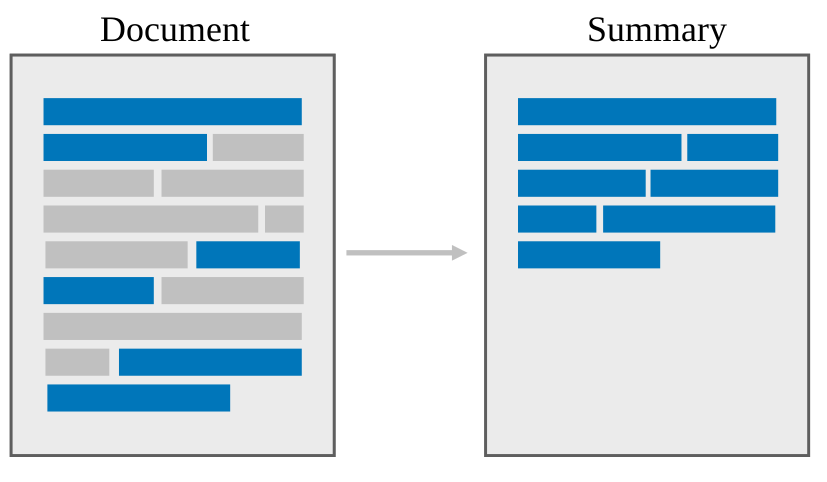
\includegraphics[width=0.65\textwidth,keepaspectratio=true]{tum-resources/images/summ_1.png}
		\label{fig:summ_1}
	\end{figure}
\end{frame}

\begin{frame}
	\frametitle{Summarization}
	\begin{figure}
		\centering
		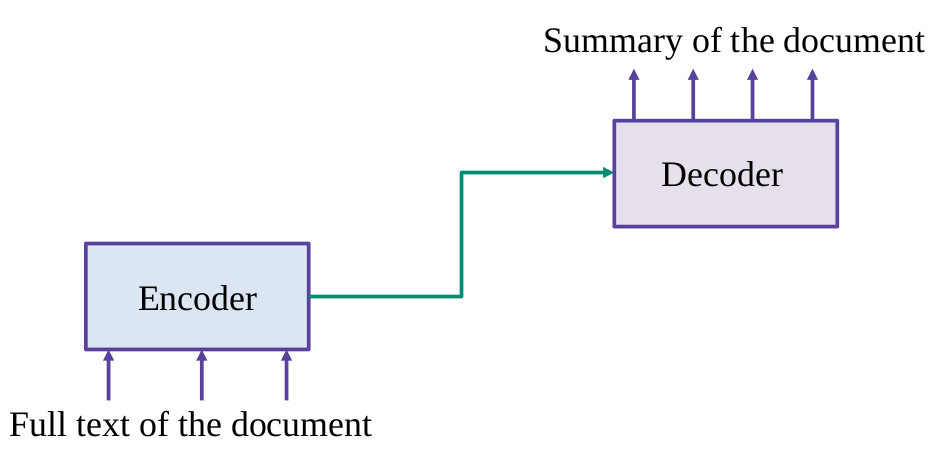
\includegraphics[width=0.65\textwidth,keepaspectratio=true]{tum-resources/images/summ_2.png}
		\label{fig:summ_2}
	\end{figure}
\end{frame}

\begin{frame}
	\frametitle{Seq2seq + attention}
	\begin{figure}
		\centering
		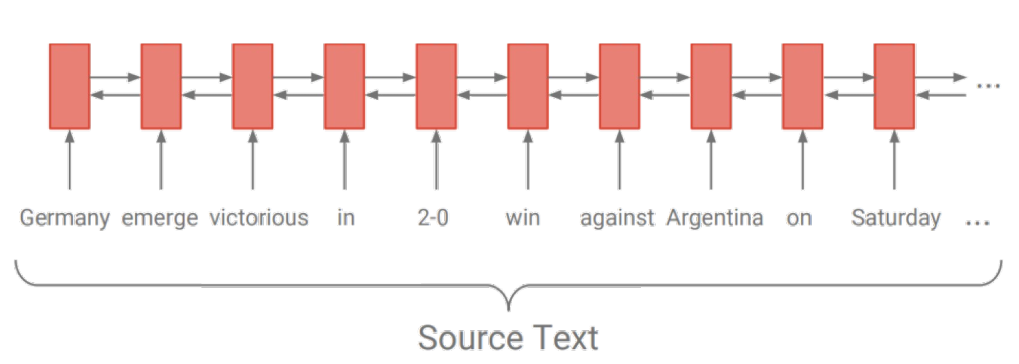
\includegraphics[width=0.65\textwidth,keepaspectratio=true]{tum-resources/images/p_summ_1.png}
		\label{fig:p_summ_1}
	\end{figure}
\end{frame}

\begin{frame}
	\frametitle{Seq2seq + attention}
	\begin{figure}
		\centering
		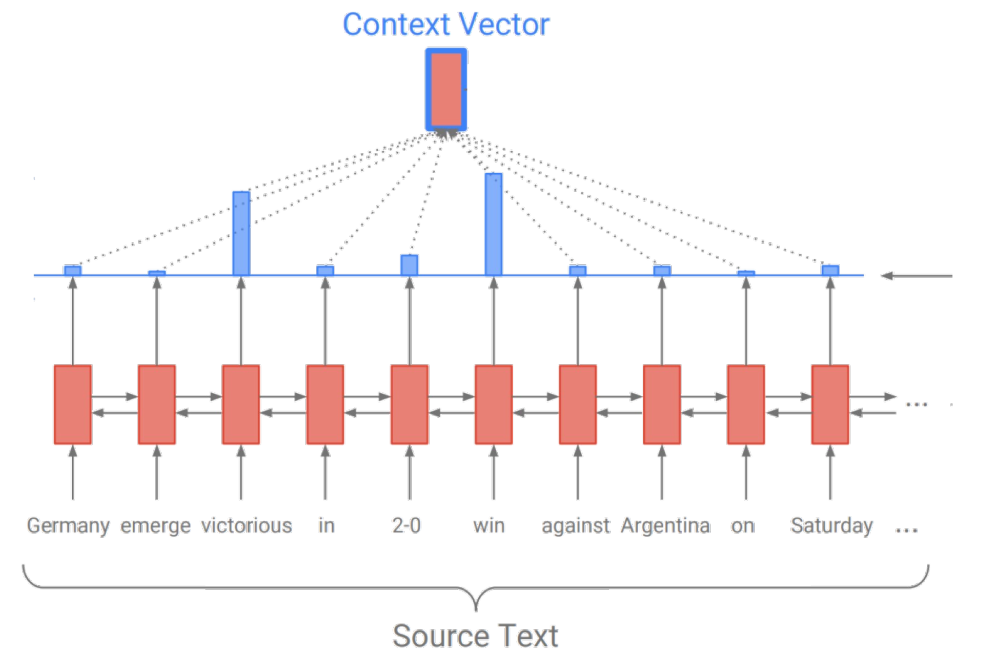
\includegraphics[width=0.65\textwidth,keepaspectratio=true]{tum-resources/images/p_summ_2.png}
		\label{fig:p_summ_2}
	\end{figure}
\end{frame}

\begin{frame}
	\frametitle{Seq2seq + attention}
	\begin{figure}
		\centering
		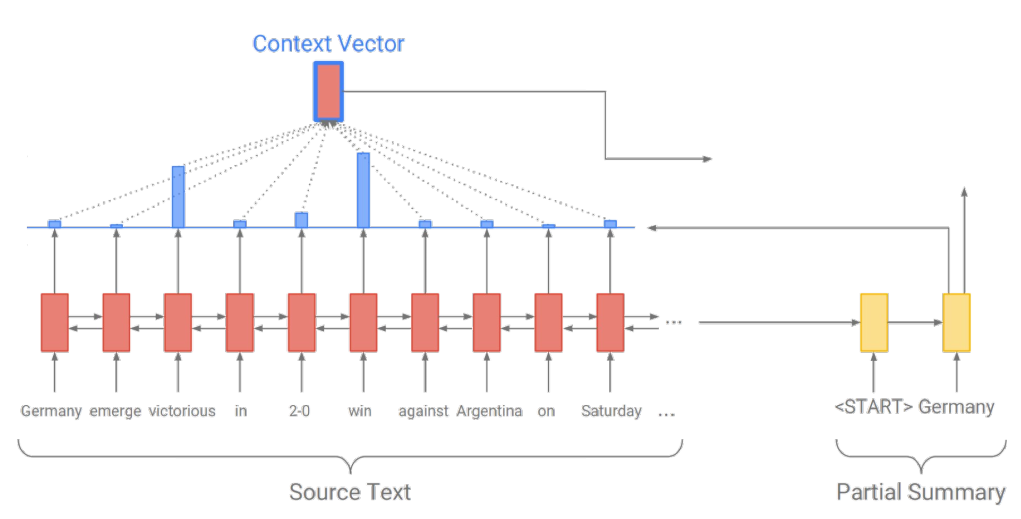
\includegraphics[width=0.65\textwidth,keepaspectratio=true]{tum-resources/images/p_summ_3.png}
		\label{fig:p_summ_3}
	\end{figure}
\end{frame}

\begin{frame}
	\frametitle{Seq2seq + attention}
	\begin{figure}
		\centering
		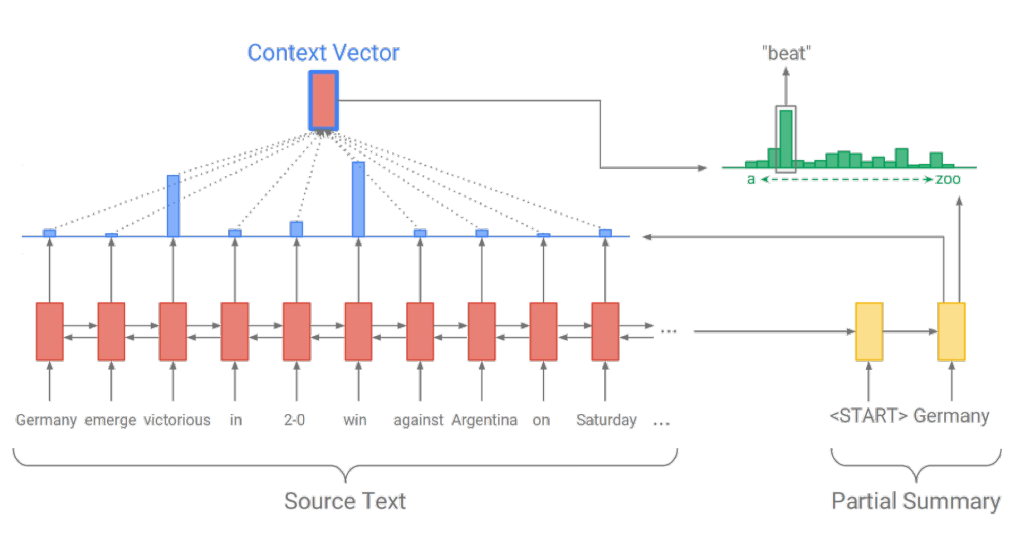
\includegraphics[width=0.65\textwidth,keepaspectratio=true]{tum-resources/images/p_summ_4.png}
		\label{fig:p_summ_4}
	\end{figure}
\end{frame}

\begin{frame}
		\huge \textbf{\textcolor{TUMBlau}{1. Attention distribution (over source positions):}}
		\vskip 0.2in
		\begin{center}
			$e_i^j = w^T \tanh(W_h h_i + W_s s_j + b_{attn})$ \\
			\vskip 0.2in
			$p^{j} = softmax(e^j)$
		\end{center}
		\vskip 0.2in
		\textbf{\textcolor{TUMBlau}{2. Vocabulary distribution (generative model):}}
		\begin{center}
			$v_j = \sum_{i} p_i^j h_i$ \\
			\vskip 0.2in
			$p_{vocab} = softmax(V^{'}(V[s_j, v_j] + b) + b^{'})$
		\end{center}
		\vskip 0.2in	
\end{frame}

\begin{frame}
	\frametitle{Copy mechanism}
	\huge What do we do with OOV words?
	\begin{figure}
		\centering
		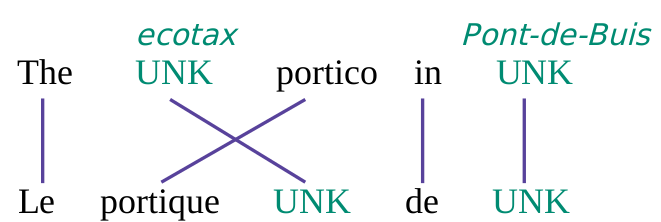
\includegraphics[width=0.65\textwidth,keepaspectratio=true]{tum-resources/images/copy_mech_1.png}
		\label{fig:copy_mech_1}
	\end{figure}
	\begin{flushright}
	\small \textit{	From "Natural Language Processing", A. Potapenko et.al. HSE, 2019. }
	\end{flushright}
\end{frame}

\begin{frame}
	\frametitle{Copy mechanism}
	\huge What do we do with OOV words?
	\begin{figure}
		\centering
		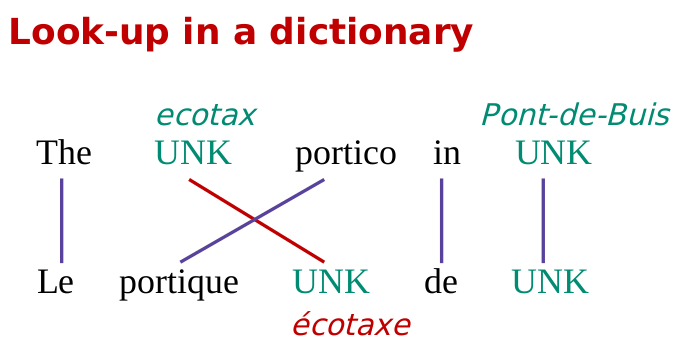
\includegraphics[width=0.65\textwidth,keepaspectratio=true]{tum-resources/images/copy_mech_2.png}
		\label{fig:copy_mech_2}
	\end{figure}
	\begin{flushright}
	\small \textit{	From "Natural Language Processing", A. Potapenko et.al. HSE, 2019. }
	\end{flushright}
\end{frame}

\begin{frame}
	\frametitle{Copy mechanism}
	\huge What do we do with OOV words?
	\begin{figure}
		\centering
		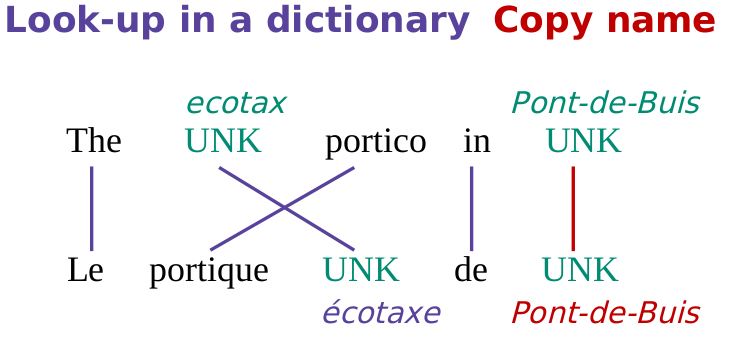
\includegraphics[width=0.65\textwidth,keepaspectratio=true]{tum-resources/images/copy_mech_3.png}
		\label{fig:copy_mech_3}
	\end{figure}
	\begin{flushright}
	\small \textit{	From "Natural Language Processing", A. Potapenko et.al. HSE, 2019. }
	\end{flushright}
\end{frame}

\begin{frame}
	\huge \textbf{\textcolor{TUMBlau}{3. Copy distribution (over words from source):}}
	\begin{center}
		$p_{copy}(w) = \sum_{i: x_i=w} p_i^{j}$
	\end{center}
	\begin{figure}
		\centering
		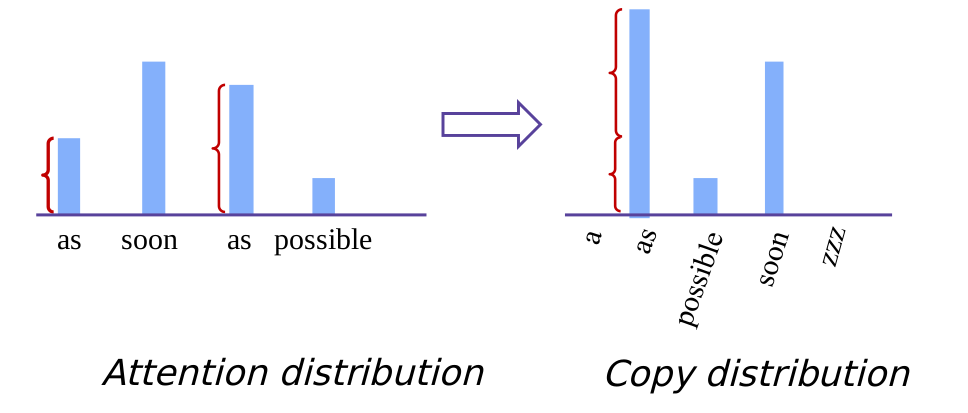
\includegraphics[width=0.65\textwidth,keepaspectratio=true]{tum-resources/images/p_summ_5.png}
		\label{fig:p_summ_5}
	\end{figure}
	\begin{flushright}
	\small \textit{	From "Natural Language Processing", A. Potapenko et.al. HSE, 2019. }
	\end{flushright}
\end{frame}

\begin{frame}
	\frametitle{Pointer-generator network}
	\begin{figure}
		\centering
		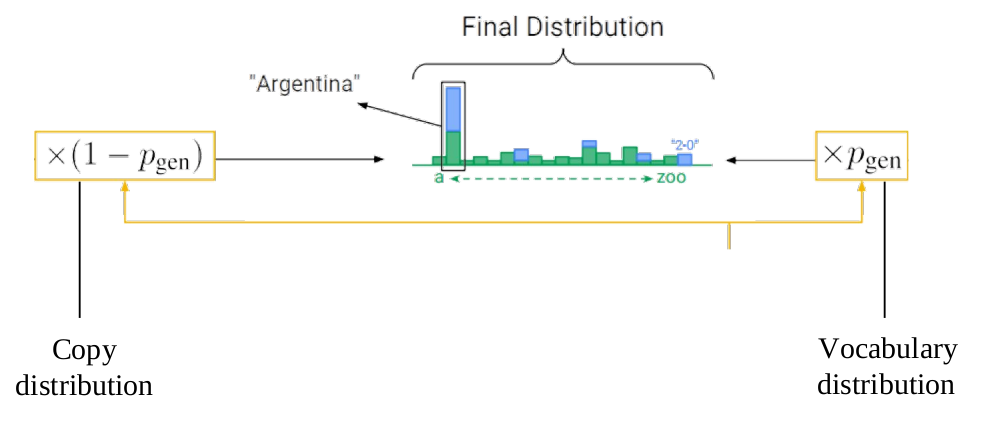
\includegraphics[width=0.65\textwidth,keepaspectratio=true]{tum-resources/images/p_summ_6.png}
		\label{fig:p_summ_6}
	\end{figure}
\end{frame}

\begin{frame}
		\huge \textbf{\textcolor{TUMBlau}{4. Final distribution:}}
		\vskip 0.2in
		\begin{center}
			$p_{final} = \textcolor{TUMOrange}{p_{gen}}p_{vocab} + \textcolor{TUMOrange}{(1-p_{gen})}p_{copy}$ \\
			\vskip 0.2in
			$\textcolor{TUMOrange}{p_{gen}} = sigmoid(w_v^T v_j + w_s^T s_j + w_x^T y_{j-1} + b_{gen})$
		\end{center}
		\vskip 0.2in
		\textbf{\textcolor{TUMBlau}{5. Training:}}
		\begin{center}
			$Loss = -\dfrac{1}{J}\sum_{j=1}^{J} \log p_{final}(y_j)$
		\end{center}
		\vskip 0.2in	
\end{frame}

\begin{frame}
	\frametitle{Pointer-generator network}
	\begin{figure}
		\centering
		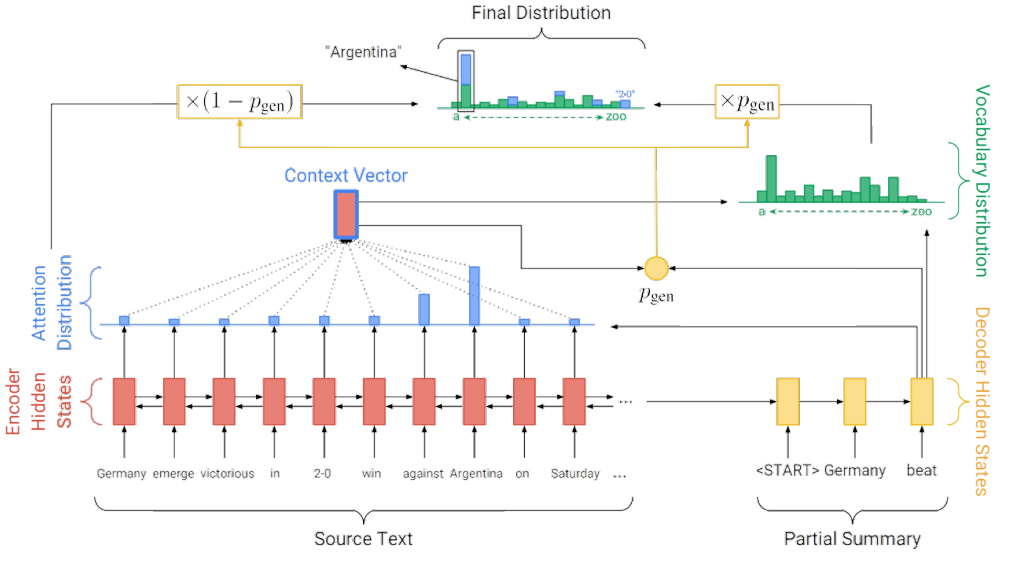
\includegraphics[width=0.65\textwidth,keepaspectratio=true]{tum-resources/images/p_summ_7.png}
		\label{fig:p_summ_7}
	\end{figure}
\end{frame}

\begin{frame}
	\frametitle{Comparison of the models}
	\begin{figure}
		\centering
		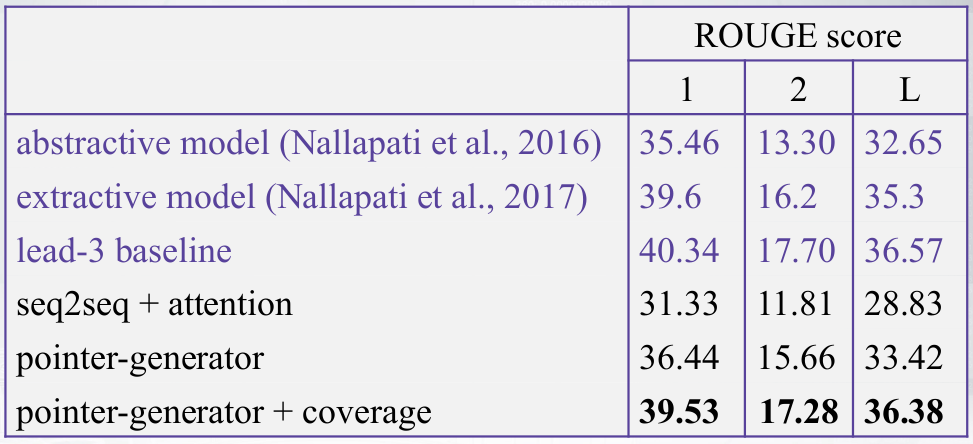
\includegraphics[width=0.65\textwidth,keepaspectratio=true]{tum-resources/images/p_summ_8.png}
		\label{fig:p_summ_8}
	\end{figure}
\end{frame}

\begin{frame}[c]
	\centering
	\begin{center}
		\Huge\textbf{Generative Adversarial Networks}
	\end{center}
\end{frame}

\begin{frame}
	\begin{figure}
		\centering
		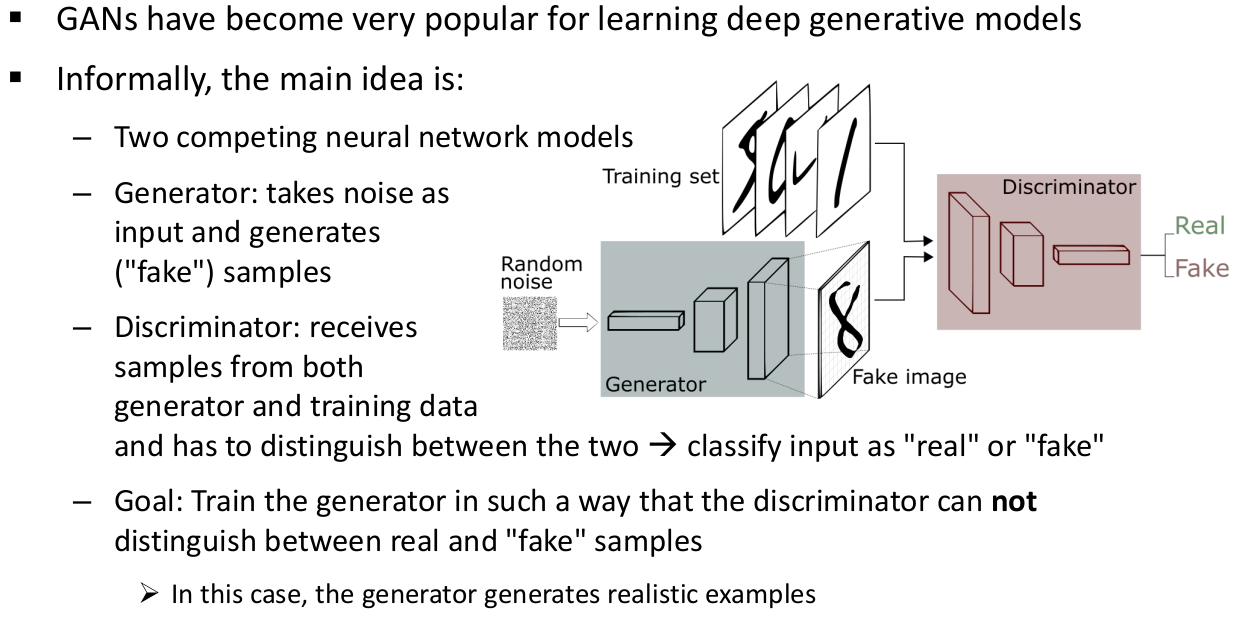
\includegraphics[width=0.85\textwidth,keepaspectratio=true]{tum-resources/images/gan_1.png}
		\label{fig:gan_1}
	\end{figure}
\begin{flushright}
\textit{	From "Mining Massive Datasets - Graphs Deep Generative Models.", Prof. Dr. Stephan Günnemann et.al. TUM, 2019. }
\end{flushright}
\end{frame}

\begin{frame}
	\begin{figure}
		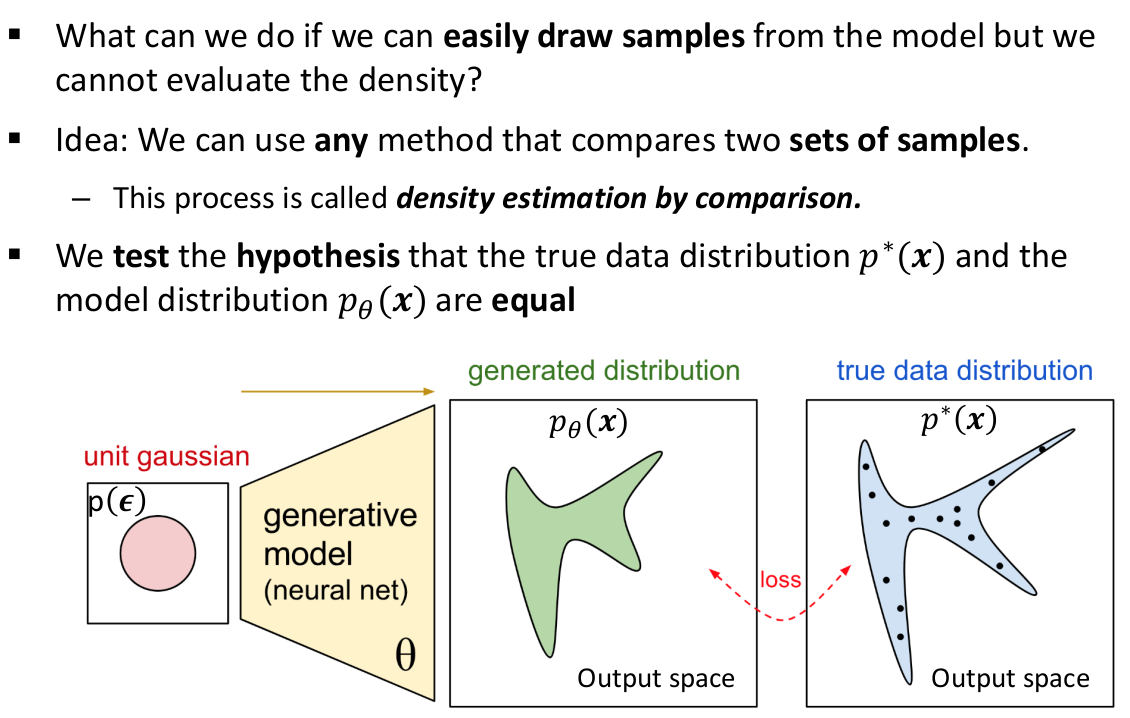
\includegraphics[width=0.70\textwidth,keepaspectratio=true]{tum-resources/images/gan_2.png}
		\label{fig:gan_2}
	\end{figure}
\begin{flushright}
	\textit{	From "Mining Massive Datasets - Graphs Deep Generative Models.", Prof. Dr. Stephan Günnemann et.al. TUM, 2019. }
\end{flushright}
\end{frame}

\begin{frame}
	\begin{figure}
		\centering
		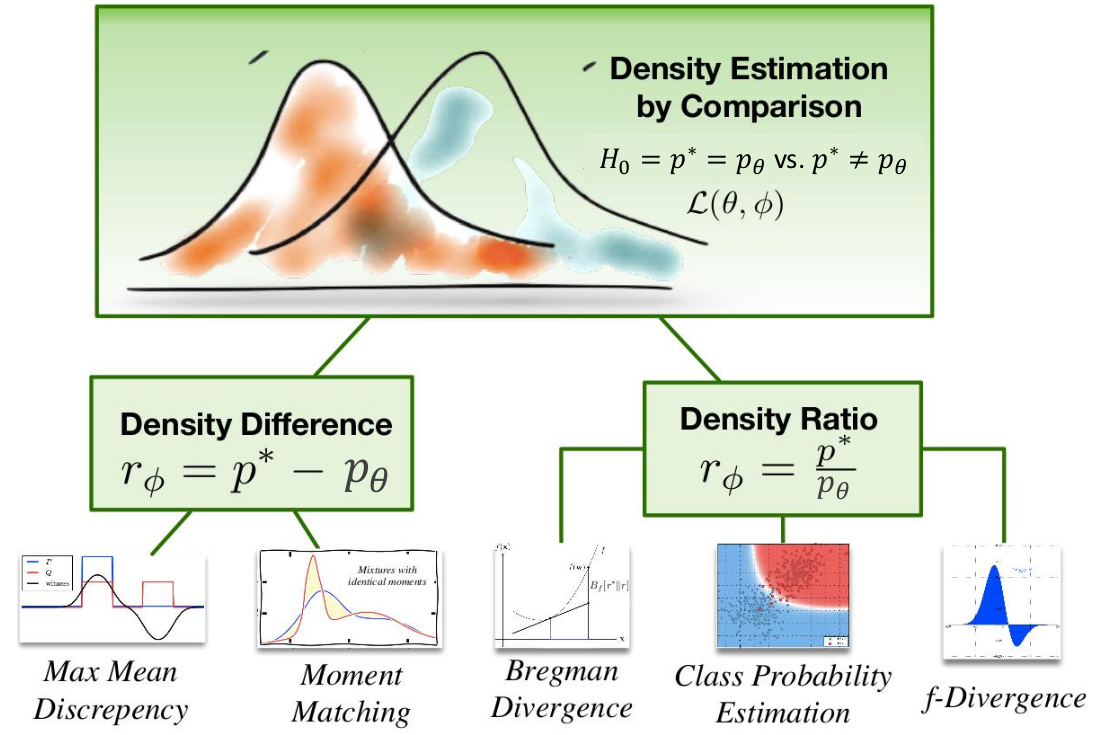
\includegraphics[width=0.65\textwidth,keepaspectratio=true]{tum-resources/images/gan_3.png}
		\label{fig:gan_3}
	\end{figure}
\begin{flushright}
	\textit{	From "Mining Massive Datasets - Graphs Deep Generative Models.", Prof. Dr. Stephan Günnemann et.al. TUM, 2019. }
\end{flushright}
\end{frame}

\begin{frame}
	\begin{figure}
		\centering
		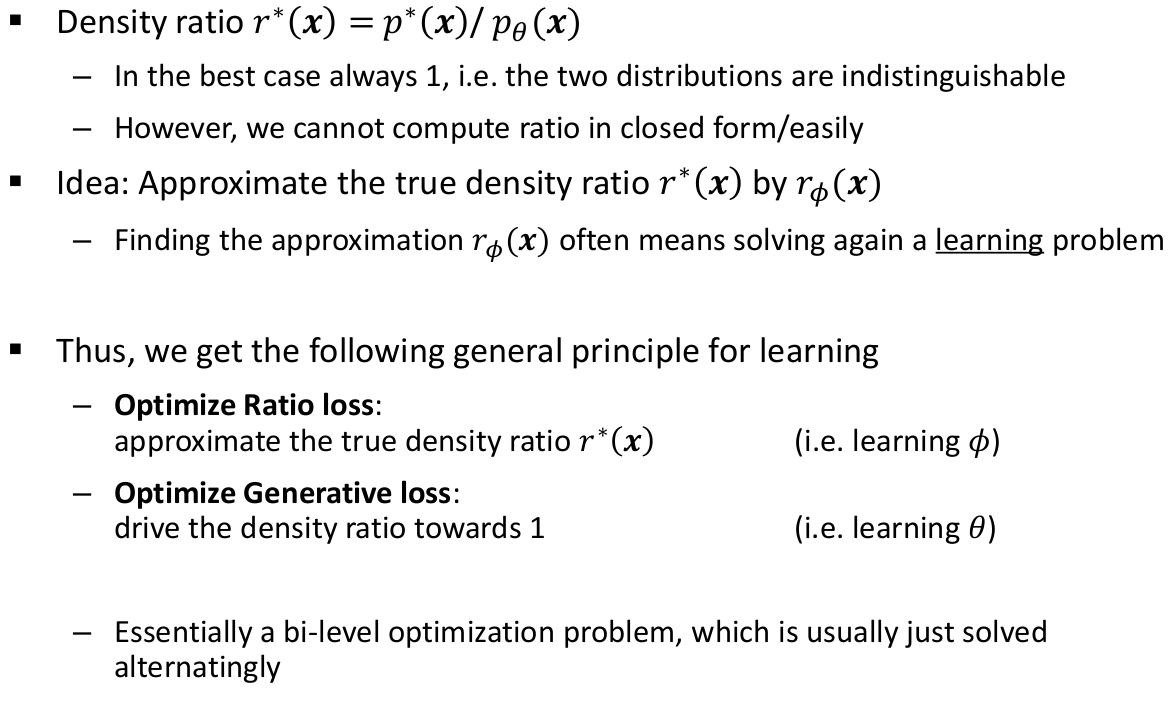
\includegraphics[width=0.75\textwidth,keepaspectratio=true]{tum-resources/images/gan_4.png}
		\label{fig:gan_4}
	\end{figure}
\begin{flushright}
	\textit{	From "Mining Massive Datasets - Graphs Deep Generative Models.", Prof. Dr. Stephan Günnemann et.al. TUM, 2019. }
\end{flushright}
\end{frame}

\begin{frame}
	\begin{figure}
		\centering
		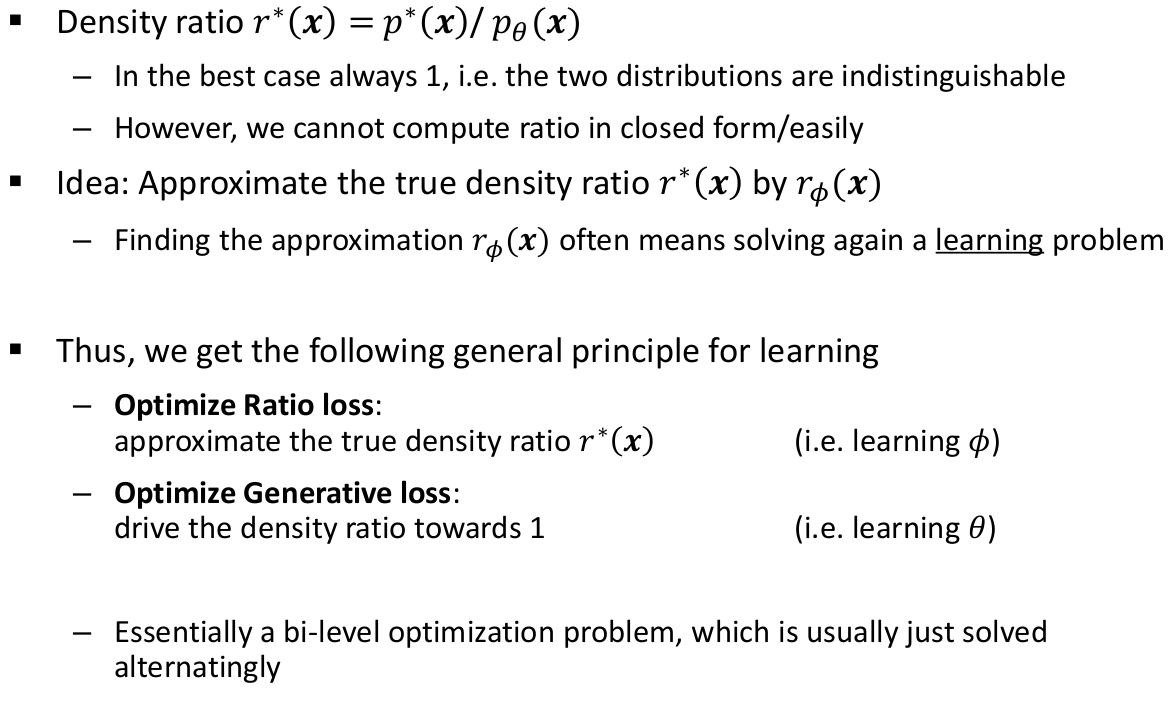
\includegraphics[width=0.75\textwidth,keepaspectratio=true]{tum-resources/images/gan_4.png}
		\label{fig:gan_4}
	\end{figure}
\begin{flushright}
	\textit{	From "Mining Massive Datasets - Graphs Deep Generative Models.", Prof. Dr. Stephan Günnemann et.al. TUM, 2019. }
\end{flushright}
\end{frame}

\begin{frame}
	\begin{figure}
		\centering
		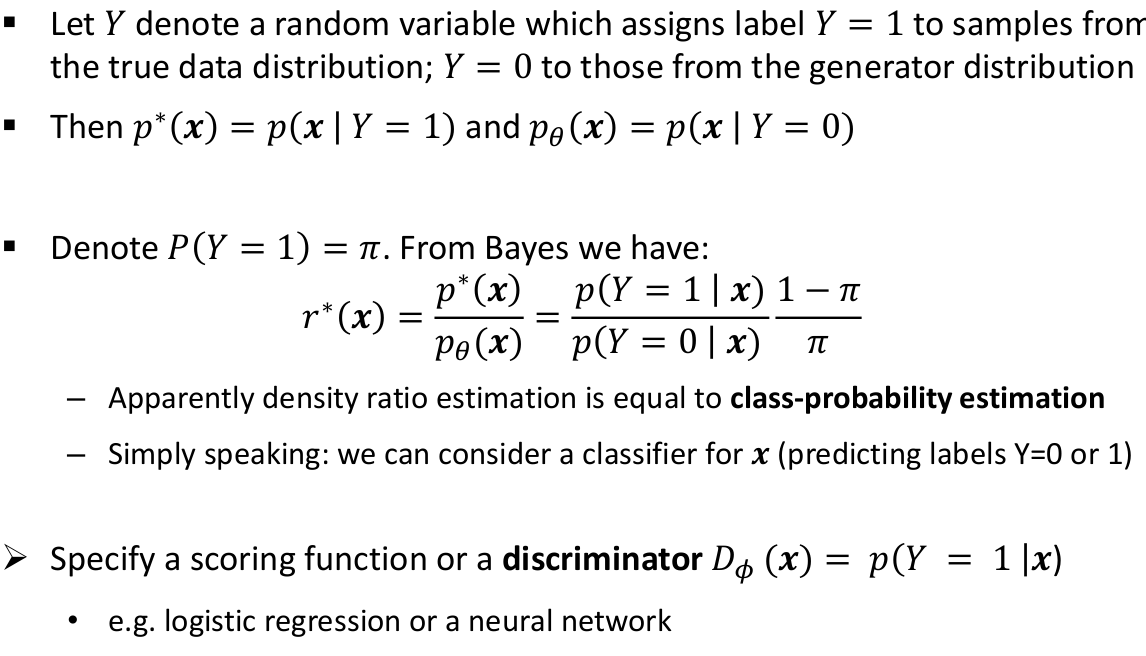
\includegraphics[width=0.75\textwidth,keepaspectratio=true]{tum-resources/images/gan_5.png}
		\label{fig:gan_5}
	\end{figure}
\begin{flushright}
	\textit{	From "Mining Massive Datasets - Graphs Deep Generative Models.", Prof. Dr. Stephan Günnemann et.al. TUM, 2019. }
\end{flushright}
\end{frame}

\begin{frame}
	\begin{figure}
		\centering
		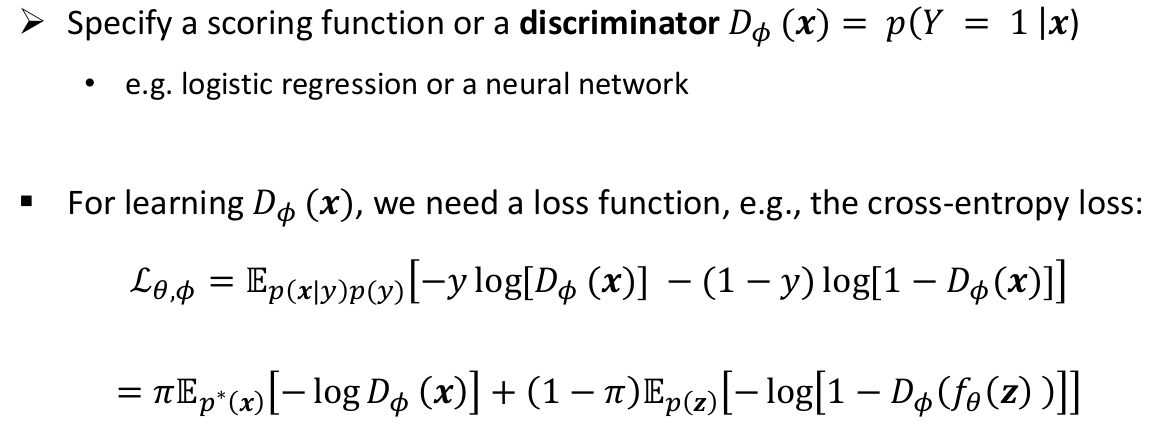
\includegraphics[width=0.8\textwidth,keepaspectratio=true]{tum-resources/images/gan_6.png}
		\label{fig:gan_6}
	\end{figure}
\begin{flushright}
	\textit{	From "Mining Massive Datasets - Graphs Deep Generative Models.", Prof. Dr. Stephan Günnemann et.al. TUM, 2019. }
\end{flushright}
\end{frame}

\begin{frame}
	\begin{figure}
		\centering
		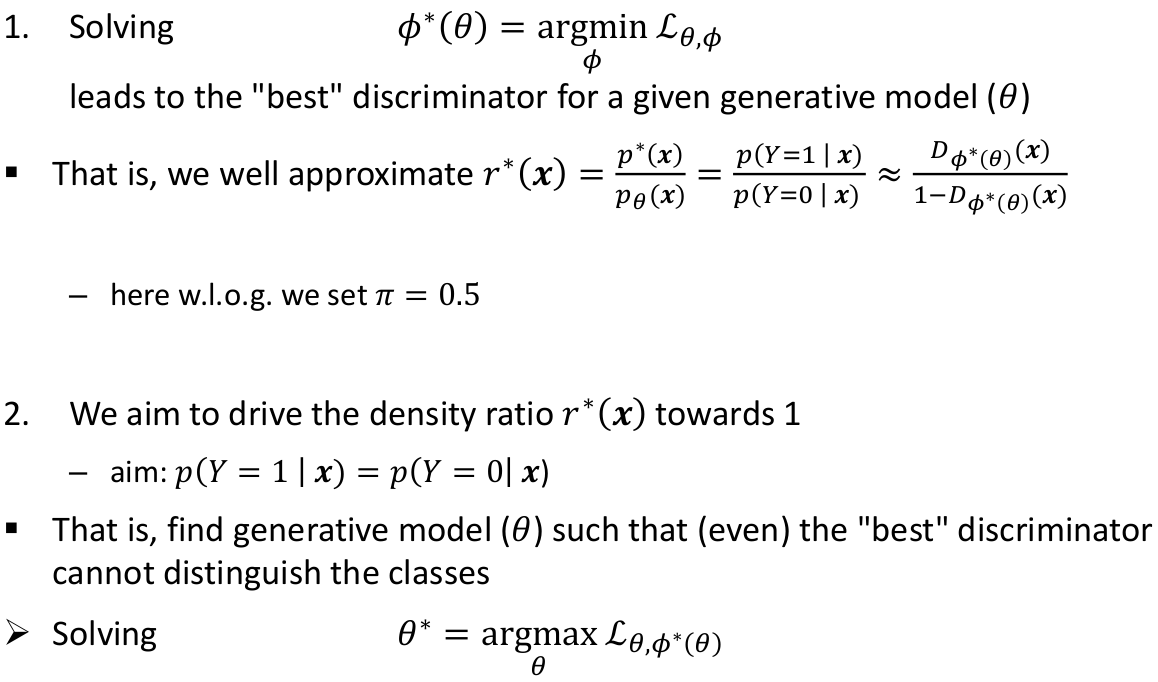
\includegraphics[width=0.75\textwidth,keepaspectratio=true]{tum-resources/images/gan_7.png}
		\label{fig:gan_7}
	\end{figure}
\begin{flushright}
	\textit{	From "Mining Massive Datasets - Graphs Deep Generative Models.", Prof. Dr. Stephan Günnemann et.al. TUM, 2019. }
\end{flushright}
\end{frame}

\begin{frame}
	\begin{figure}
		\centering
		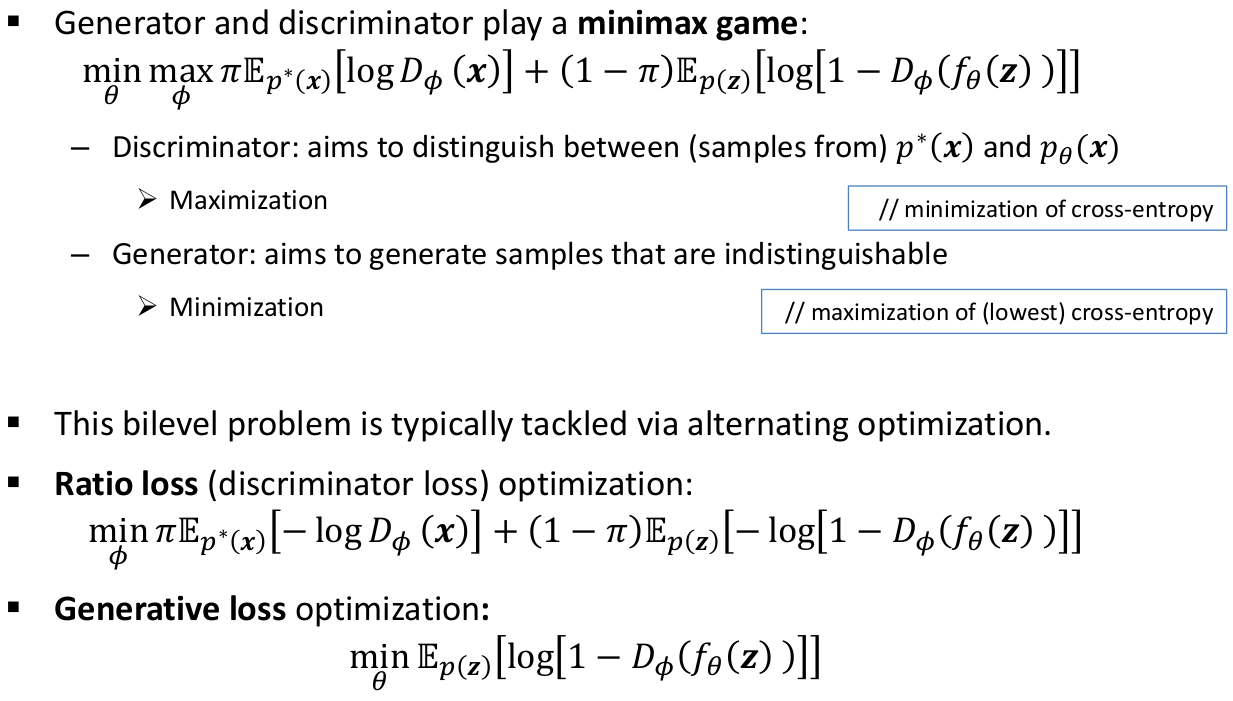
\includegraphics[width=0.75\textwidth,keepaspectratio=true]{tum-resources/images/gan_8.png}
		\label{fig:gan_8}
	\end{figure}
\begin{flushright}
	\textit{	From "Mining Massive Datasets - Graphs Deep Generative Models.", Prof. Dr. Stephan Günnemann et.al. TUM, 2019. }
\end{flushright}
\end{frame}

\begin{frame}[c]
	\centering
	\begin{center}
		\Huge\textbf{Wasserstein Generative Adversarial Networks}
	\end{center}
\end{frame}

\begin{frame}
	\begin{figure}
		\centering
		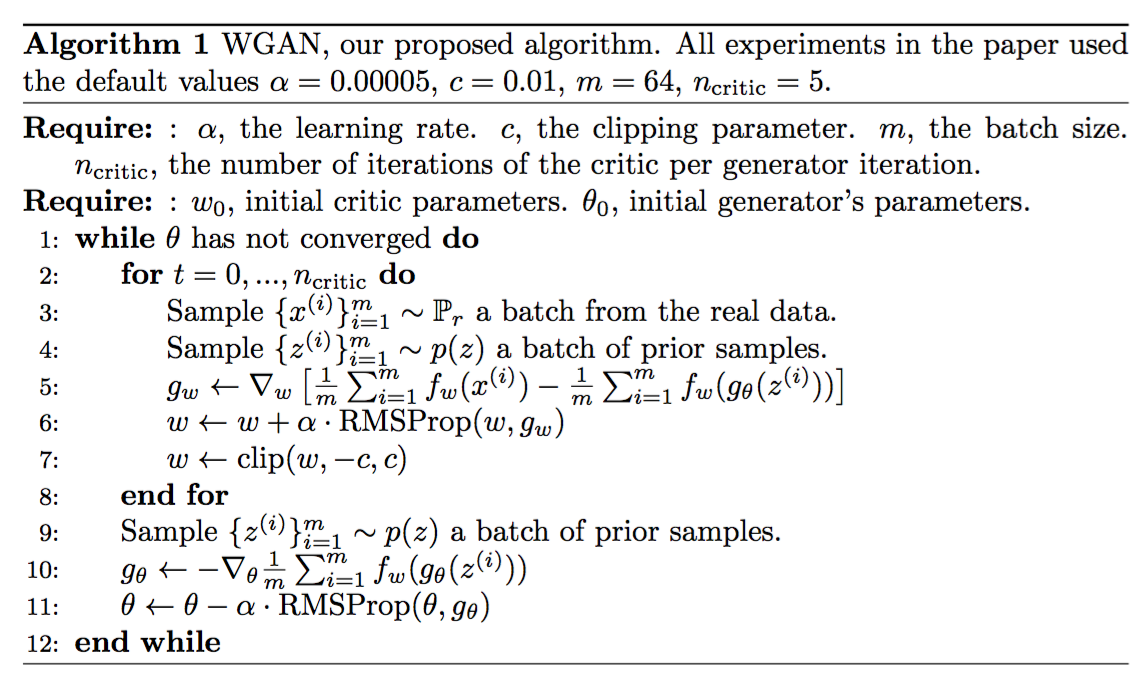
\includegraphics[width=0.75\textwidth,keepaspectratio=true]{tum-resources/images/wgan_1.png}
		\label{fig:wgan_1}
	\end{figure}
	\begin{flushright}
		\textit{Image source: Arjovsky, Chintala,  Bottou, 2017.}
	\end{flushright}
\end{frame}

\begin{frame}
	\frametitle{Wasserstein distance}
	\large Wasserstein Distance is a measure of the distance between two probability distributions. It is also called Earth Mover’s distance. It can be interpreted as the minimum energy cost of moving and transforming a pile of dirt in the shape of one probability distribution to the shape of the other distribution. 
	\vskip 0.2in
	\begin{figure}
		\centering
		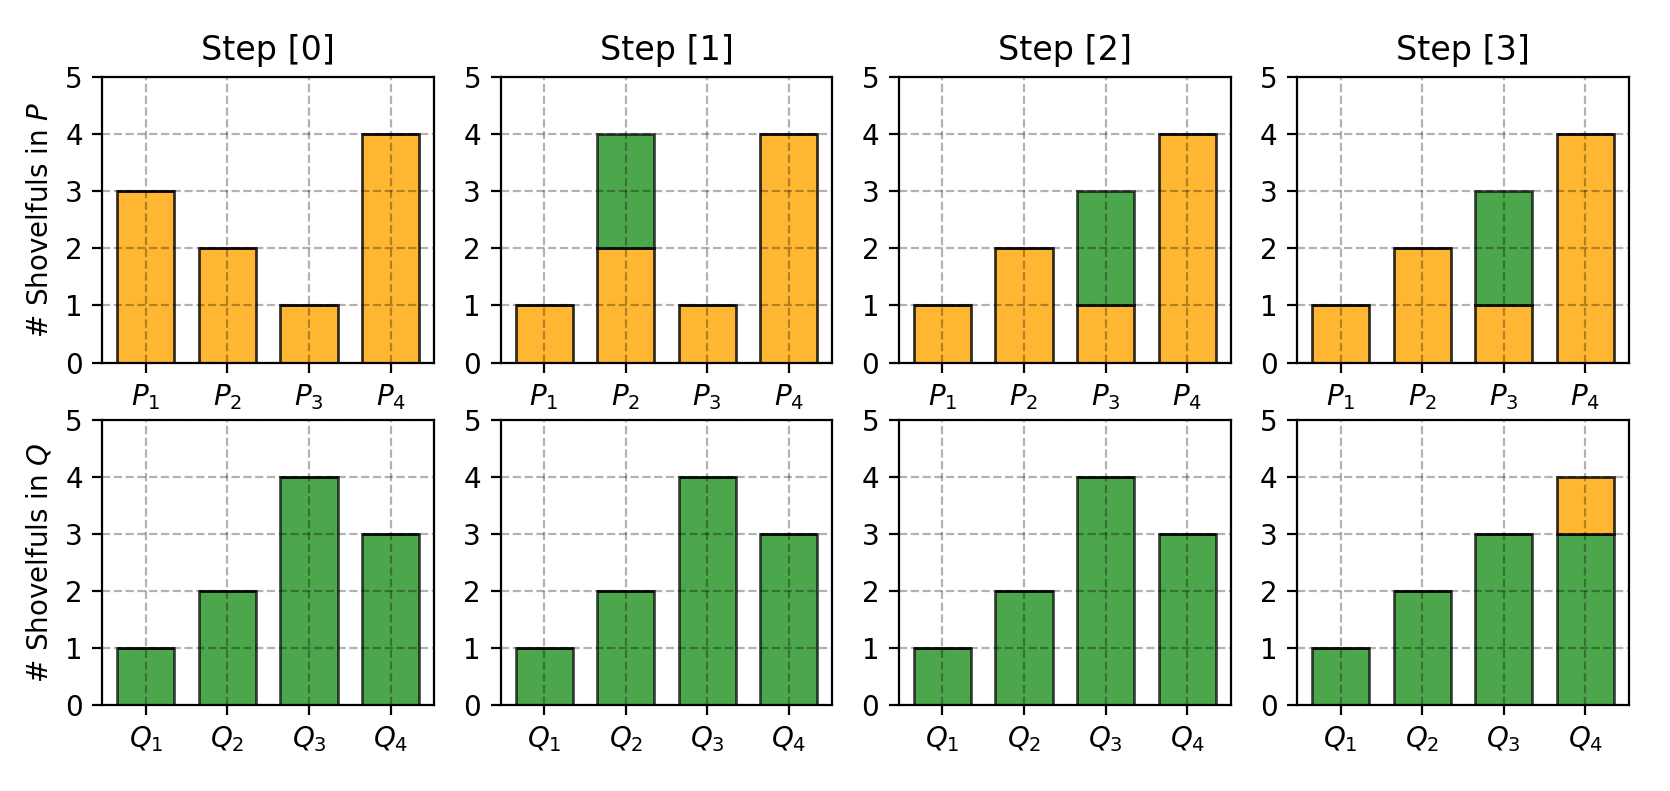
\includegraphics[width=0.6\textwidth,keepaspectratio=true]{tum-resources/images/wgan_2.png}
		\label{fig:wgan_2}
	\end{figure}
\begin{flushright}
	\textit{	From "https://arxiv.org/pdf/1904.08994.pdf". }
\end{flushright}
\end{frame}

\begin{frame}
\begin{center}
	$ P_1 = 3, P_2 = 2, P_3 = 1, P_4 = 4 $ \\
	$ Q_1 = 1, Q_2 = 2, Q_3 = 4, Q_4 = 3$
\end{center}
If we label the cost to pay to make $P_i$ and $Q_i$ match $\delta_i$, we would have $\delta_{i+1} = \delta_i + P_i - Q_i$
and in example:
\begin{center}
	\begin{equation}	
	% <![CDATA[
	\begin{aligned}
	\delta_0 &= 0\\
	\delta_1 &= 0 + 3 - 1 = 2\\
	\delta_2 &= 2 + 2 - 2 = 2\\
	\delta_3 &= 2 + 1 - 4 = -1\\
	\delta_4 &= -1 + 4 - 3 = 0
	\end{aligned} %]]>
	\end{equation}
\end{center}
\large When dealing with the continuous probability domain, the distance formula becomes:
\begin{equation}
W(p^{*}(x), p(z)) = \inf_{\gamma \sim \Pi(p^{*}(x), p(z))} \mathbb{E}_{(x, y) \sim \gamma}[\| x-y \|]
\end{equation}
	\begin{flushright}
		\textit{Image source: https://arxiv.org/pdf/1904.08994.pdf".}
	\end{flushright}
\end{frame}

\begin{frame}
	\frametitle{Why Wasserstein is better than JS or KL divergence?}
	Suppose we have two probability distributions, $P$ and $Q$:
	\begin{equation}
		\begin{aligned}
			\forall (x, y) \in P, x = 0 \text{ and } y \sim U(0, 1) \\
			\forall (x, y) \in Q, x = \theta, 0 \leq \theta \leq 1 \text{ and } y \sim U(0, 1)
		\end{aligned}
	\end{equation}
	\begin{figure}
		\centering
		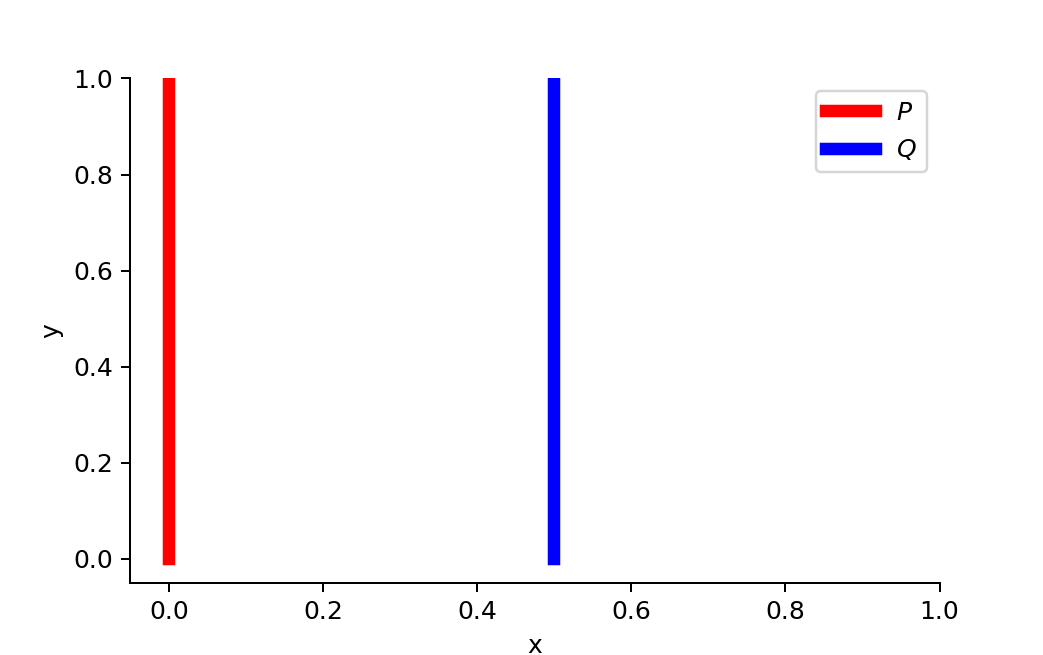
\includegraphics[width=0.55\textwidth,keepaspectratio=true]{tum-resources/images/wgan_3.png}
		\label{fig:wgan_3}
	\end{figure}
	\begin{flushright}
		\textit{From "https://arxiv.org/pdf/1904.08994.pdf".}
	\end{flushright}
\end{frame}

\begin{frame}
	\begin{equation}
	% <![CDATA[
		\begin{aligned}
			D_{KL}(P \| Q) &= \sum_{x=0, y \sim U(0, 1)} 1 \cdot \log\frac{1}{0} = +\infty \\
			D_{KL}(Q \| P) &= \sum_{x=\theta, y \sim U(0, 1)} 1 \cdot \log\frac{1}{0} = +\infty \\
			D_{JS}(P, Q) &= \frac{1}{2}(\sum_{x=0, y \sim U(0, 1)} 1 \cdot \log\frac{1}{1/2} + \sum_{x=0, y \sim U(0, 1)} 1 \cdot \log\frac{1}{1/2}) = \log 2\\
			W(P, Q) &= |\theta|
		\end{aligned} %]]>
	\end{equation}
	But when $\theta = 0$, two distributions are fully overlapped:
	\begin{equation}
		% <![CDATA[
		\begin{aligned}
		D_{KL}(P \| Q) &= D_{KL}(Q \| P) = D_{JS}(P, Q) = 0\\
		W(P, Q) &= 0 = \lvert \theta \rvert
		\end{aligned} %]]>
	\end{equation}
	\begin{flushright}
		\textit{From "https://arxiv.org/pdf/1904.08994.pdf".}
	\end{flushright}
\end{frame}

\begin{frame}
	\frametitle{The differences in implementation for the WGAN}
	\begin{enumerate}
		\item Use a linear activation function in the output layer of the critic model (instead of sigmoid).
		\item Use -1 labels for real images and 1 labels for fake images (instead of 1 and 0).
		\item Use Wasserstein loss to train the critic and generator models.
		\item Constrain critic model weights to a limited range after each mini batch update (e.g. [-0.01,0.01]).
		\item Update the critic model more times than the generator each iteration (e.g. 5).
		\item Use the RMSProp version of gradient descent with a small learning rate and no momentum (e.g. 0.00005).	
	\end{enumerate}
	\begin{flushright}
		\textit{From "https://arxiv.org/pdf/1904.08994.pdf".}
	\end{flushright}
\end{frame}

\begin{frame}[c]
	\centering
	\begin{center}
		\Huge\textbf{Putting all together}
	\end{center}
\end{frame}

\begin{frame}
	\begin{figure}
		\centering
		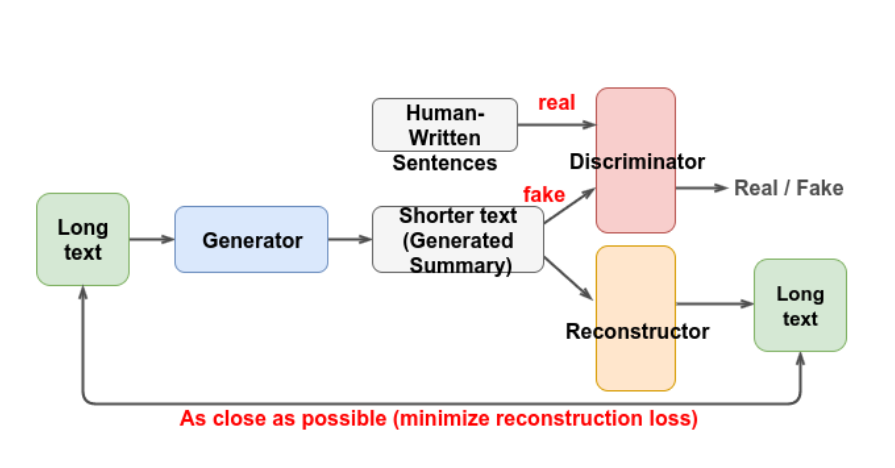
\includegraphics[width=0.8\textwidth,keepaspectratio=true]{tum-resources/images/paper_2.png}
		\label{fig:paper_2}
	\end{figure}
\end{frame}

\begin{frame}
	\begin{figure}
		\centering
		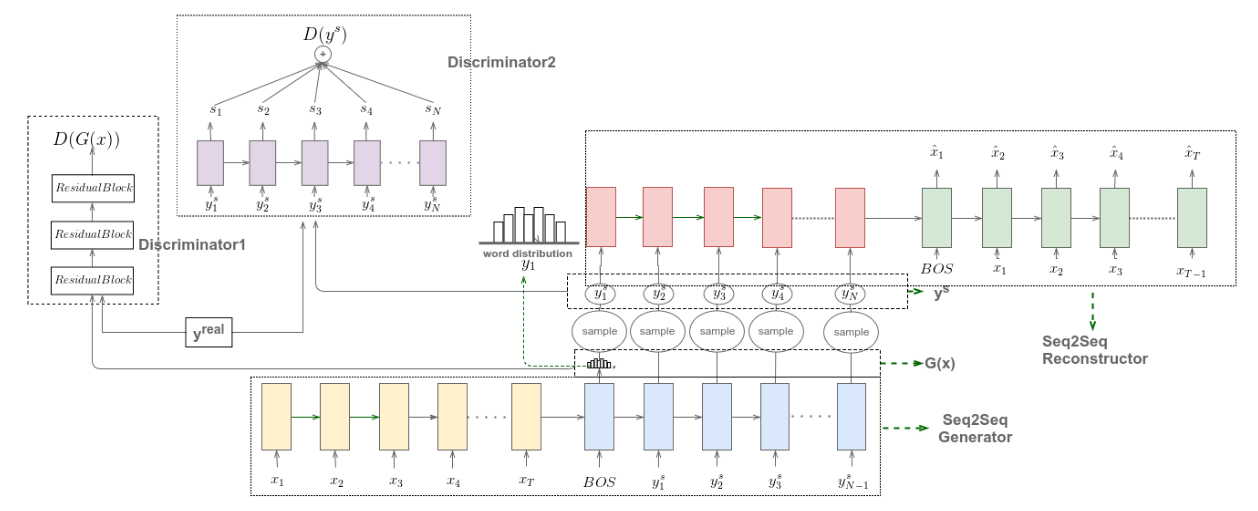
\includegraphics[width=1\textwidth,keepaspectratio=true]{tum-resources/images/paper_3.png}
		\label{fig:paper_3}
	\end{figure}
\end{frame}

\begin{frame}
	\frametitle{Key learnings from the paper}
	\begin{itemize}
		\item Keras very flexible framework which is underestimated in community
		\item Keras and tensorflow is very unstable from version to version
		\item migration from python2 to python3 is nightmare 
	\end{itemize}
\end{frame}

\begin{frame}
	\frametitle{Critics of authors}
	\begin{itemize}
		\item Paper is very bad detiled, there are missed part
		\item Code provided by authors is hardly reprodusable and not documented
		\item ...
	\end{itemize}
\end{frame}

\begin{frame}
	\frametitle{Thank you for your attention}
	\framesubtitle{Any questions?}
\end{frame}

\begin{frame}
	\frametitle{References}
	\printbibliography
\end{frame}

\end{document}
